\section{O sistema que foi convertido}
\label{sec:sistema}

O SIS Eventos serve para a instituição registrar os eventos em que quer participar, como congressos e feiras, e prever quanto vai gastar com cada um. O sistema tem duas partes: o aplicativo, feito em Power Apps (ferramenta da Microsoft para criar aplicativos por telas), e as listas do SharePoint, que funcionam como tabelas de um banco de dados e guardam as informações.

O uso começa na tela de exercícios (Figura~\ref{fig:tela-exercicios}), onde o usuário escolhe o ano. Em seguida, a tela de solicitações (Figura~\ref{fig:tela-solicitacoes}) mostra os eventos daquele ano, com a situação de cada um, como aprovado, em análise ou cancelado, e o custo previsto. Ao abrir um evento, aparecem os itens de custo: diárias, inscrição, passagem e seguro (Figura~\ref{fig:tela-custos}).

Os dados ficam em listas ligadas entre si. Cada evento tem vários itens de custo, e cada item de custo usa um valor de diária de outra lista (Figura~\ref{fig:listas}). As regras estudadas ficam nas fórmulas dos componentes das telas, escritas em Power Fx, a linguagem de fórmulas do Power Apps. Por isso, para converter uma regra, o agente precisa achar a fórmula certa dentro da tela e entender de quais listas ela depende.

\begin{figure}[htbp]
\centering
\caption{Tela de exercícios}
\label{fig:tela-exercicios}
\fbox{\parbox[c][4cm][c]{0.85\textwidth}{\centering\textbf{[FIGURA PENDENTE: tela de exercícios do app com dados inventados. Print da Anna.]}}}
\end{figure}

\begin{figure}[htbp]
\centering
\caption{Tela de solicitações}
\label{fig:tela-solicitacoes}
\fbox{\parbox[c][4cm][c]{0.85\textwidth}{\centering\textbf{[FIGURA PENDENTE: tela de solicitações. Print da Anna.]}}}
\end{figure}

\begin{figure}[htbp]
\centering
\caption{Tela com os itens de custo de um evento}
\label{fig:tela-custos}
\fbox{\parbox[c][4cm][c]{0.85\textwidth}{\centering\textbf{[FIGURA PENDENTE: tela com os itens de custo de um evento. Print da Anna.]}}}
\end{figure}

\begin{figure}[htbp]
\centering
\caption{Listas do sistema e como se ligam}
\label{fig:listas}
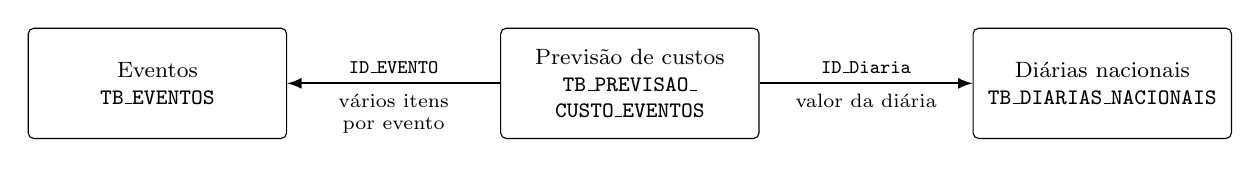
\begin{tikzpicture}[
    lista/.style={draw, rounded corners=2pt, align=center, font=\footnotesize,
                  text width=3cm, minimum height=1.4cm, inner sep=4pt},
    liga/.style={-latex, thick},
    rotulo/.style={font=\scriptsize, align=center}
]
\node[lista] (ev) at (0,0)  {Eventos\\\texttt{TB\_EVENTOS}};
\node[lista] (pc) at (6,0)  {Previsão de custos\\\texttt{TB\_PREVISAO\_\allowbreak CUSTO\_EVENTOS}};
\node[lista] (dn) at (12,0) {Diárias nacionais\\\texttt{TB\_DIARIAS\_\allowbreak NACIONAIS}};
\draw[liga] (pc) -- node[rotulo, above] {\texttt{ID\_EVENTO}} node[rotulo, below] {vários itens\\por evento} (ev);
\draw[liga] (pc) -- node[rotulo, above] {\texttt{ID\_Diaria}} node[rotulo, below] {valor da diária} (dn);
\end{tikzpicture}
\\[2pt]
\footnotesize Fonte: elaborado pela autora.
\end{figure}

\subsection{Como as quatro regras funcionam}
\label{sec:como-regras}

Esta subseção descreve as regras como elas foram lidas nas fórmulas do sistema, no editor do Power Apps. Elas são a base para os testes do estudo de caso.

\textbf{Registros excluídos.} As listas têm um campo, isto é, uma coluna, chamado \texttt{Excluido}. Os eventos, os custos e as diárias marcados com um asterisco (*) nesse campo são ignorados nas regras 01, 03 e 04. A regra 02 não olha esse campo: ela calcula o valor da linha de custo mesmo quando a linha está excluída, e usa o valor da diária da lista mesmo quando a diária está excluída.

\textbf{Regra 01: eventos por ano.} A regra 01 conta os eventos de cada ano, no total e por status, sem os eventos excluídos. O status é a situação do pedido: Em Aberto, Em Análise, Aprovado, Não Aprovado, Cancelado ou Aprovado para ajustes.

\textbf{Diárias nacionais.} A diária é o valor pago por dia de viagem. Em um evento nacional, a pessoa escolhe o cargo ou função. O sistema então mostra as diárias da lista de diárias nacionais que têm a mesma classificação desse cargo. Cada opção aparece com o nome da cidade ou capital e o valor da diária. A classe do cargo é preenchida automaticamente a partir da lista de cargos. Se o âmbito do evento não for nacional, essa lista não mostra opções.

\textbf{Regra 02: valor de cada linha de custo.} Cada linha de custo é um gasto previsto do evento, como uma passagem ou uma inscrição. O valor da linha depende do tipo de custo. O sistema testa os casos na ordem abaixo e usa o primeiro que se aplica. O resultado aparece em reais.

\begin{itemize}
    \item seguro viagem: valor do seguro $\times$ quantidade de pessoas;
    \item diária internacional: o valor já convertido para reais, guardado na linha;
    \item passagem: quantidade de pessoas $\times$ passagem individual;
    \item diária de outro cargo, com o valor digitado à mão: quantidade de diárias $\times$ valor digitado $\times$ quantidade de pessoas;
    \item diária nacional, com o valor da lista: quantidade de diárias $\times$ valor da diária;
    \item inscrição: o valor já convertido para reais, guardado na linha;
    \item custo complementar: o próprio valor.
\end{itemize}

\textbf{Regra 03: total previsto de custos.} A regra 03 calcula o total previsto de custos dos eventos aprovados de um ano. Para cada evento aprovado, ela soma as linhas de custo previstas que não foram excluídas. Cada linha soma sete partes:

\begin{itemize}
    \item diária de outro cargo: quantidade de diárias $\times$ valor digitado $\times$ quantidade de pessoas;
    \item diária nacional: quantidade de diárias $\times$ valor da lista $\times$ quantidade de pessoas;
    \item diária internacional: cotação do dólar, isto é, quanto um dólar vale em reais, $\times$ valor em dólar $\times$ quantidade de diárias $\times$ quantidade de pessoas;
    \item inscrição: o valor, multiplicado pela cotação do dólar quando a moeda é o dólar;
    \item custo complementar: o próprio valor;
    \item seguro viagem: valor $\times$ quantidade de pessoas;
    \item passagem: passagem individual $\times$ quantidade de pessoas.
\end{itemize}

Cada parte é arredondada para duas casas decimais, ou seja, até os centavos, e o total aparece em reais. Essa conta soma todos os campos da linha, sem olhar o tipo de custo.

\textbf{Regra 04: total realizado.} O valor realizado é o que foi de fato gasto, guardado no campo \texttt{Realizado}. A regra 04 mostra o total realizado dos eventos aprovados de um ano. Ela soma o campo \texttt{Realizado} das linhas de custo que não foram excluídas, dos eventos aprovados e não excluídos daquele ano. As linhas com o campo \texttt{Realizado} vazio ficam de fora da soma.
